\section{Dataset}

Our analysis is based on \num{2204199} alias definitions found on GitHub, collected over a period of two-and-a-half weeks from December 20th 2019 to January 8th 2020.

\subsection{Data Collection}

\begin{figure*}
	\centering
	%\vspace{2em}
	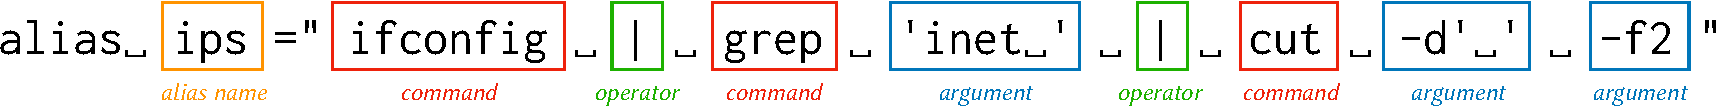
\includegraphics[width=0.85\textwidth]{figures/parser_breakdown.pdf}
	\cprotect\caption{Decomposition of \verb`alias ips="ifconfig | grep 'inet ' | cut -d' ' -f2"`.}
	\label{fig:parser}
\end{figure*}

Alias definitions can appear in any Shell script, but we anticipated that they would predominantly be found in personal configuration files (like \verb|.bashrc| or \verb|.bash_profile|).
%While we did not want to focus exclusively on these personal configuration scripts, as we want to study the wide range of different alias uses, it is important that they are appropriately accounted for in order for our data to be representative.
Unfortunately, this rules out using some prominent existing datasets for our study~\cite{mombach}:
The public GitHub archive on BigQuery,\footnote{\url{https://bigquery.cloud.google.com/table/bigquery-public-data:github_repos.files}} while containing over 1.5 TB of source code, only includes ``notable projects'' (presumably those with a certain number of stars on GitHub) that additionally have an explicit open source license. 
This leaves out many of the repositories we are interested in, as users sharing configuration scripts for personal use do not usually add a license file and their repositories are generally not ``notable''.
GHTorrent~\cite{ghtorrent}, another popular archive of GitHub data, only contains metadata but not file contents.

Therefore, we found it necessary to write our own tooling to directly collect the data from GitHub ourselves.
We used the GitHub Code Search API to find files written in Shell language\footnote{GitHub uses the Linguist library to classify code: \url{https://github.com/github/linguist}} that contain the string \verb|alias|.

Alas, the GitHub Code Search API comes with its own set of limitations:
\begin{enumerate}
    \item only files smaller than 384 KB are searchable
    \item forks are not included
    \item requests are rate limited at 30 per minute and there are additional opaque abuse detection mechanisms that impose further restrictions in an unforeseeable manner
    \item the number of results is limited to \num{1000} per search request
\end{enumerate}
The first two limitations do not really affect us, as we are interested in smaller files and do not have to consider forks.
The rate limiting, while significantly slowing down the retrieval process, is also not a fatal obstacle.
The maximum number of returned search results, however, is a critical limitation.
To get around it, we wrote a Python tool called \verb|BLINDED-SEARCHER| that uses a clever sampling strategy to vastly increase the number of results we are able to retrieve.
% \verb|github-searcher|\footnote{\TODO: url/paper} 

The sampling strategy is based on the GitHub API allowing code search queries to be conditioned on file sizes. 
For example, the query 
\begin{CVerbatim}
alias language:Shell size:101..200
\end{CVerbatim}
returns up to \num{1000} Shell language files containing the string ``alias'' that have a file size between 101 and 200 bytes (inclusive).
Repeating the search with 
\begin{CVerbatim}
alias language:Shell size:201..300
\end{CVerbatim}
returns up to \num{1000} files of a size between 201 and 300 bytes, and so on.
Repeatedly searching with the same search term but different non-overlapping file size ranges allows us to significantly increase our sample of the overall population.
Another trick further improves on this: 
the API gives us an option to sort the results by most or least recently indexed;
if we run a search using a specific sort order, then we can effectively double the sample size by repeating the same search with the opposite sort order.
Thus we can get up to \num{2000} results per search per file size range.

Additionally, while GitHub does not allow us to retrieve more than a limited number of files per query, it does return the total count of files matching the query.
While this count is usually very erratic on broad searches, fluctuating wildly between repeated requests, it turns out to be fairly accurate for searches with a small number of results, such as those conditioned on a narrow range of file sizes.
This allows us to get a good estimate of the population, and how accurately our sample approximates it.

For this study, using the search term
\begin{CVerbatim}
alias language:Shell
\end{CVerbatim}
and the sampling strategy described above, we started by sampling all files in increments of 100 bytes and stopped when we reached 29 KB.
We then re-sampled some high-population areas with smaller size increments in order to get a better sample, in some cases sampling in increments of 1 byte.
In total, we collected \num{844140} files from \num{304361} GitHub repositories.
Our sample represents \per{94.09} of the estimated population of \num{897182} files under 29 KB on GitHub written in Shell language and containing the word ``alias''.
The file contents, together with repository metadata, were stored in an SQLite database.
After removing duplicates, our database contains \num{372816} unique files from \num{205126} repositories.

% NOTE: this table is from the next section, but the LaTeX gods demand I place it here
\begin{table*}[!ht]
    \centering
    \caption{Top alias names, commands and arguments}
    \label{tab:top-summary}
    \begin{tabular}{lrr}
\toprule
   Alias Name &           \# &          \% \\
\midrule
    \verb|ls| &  \num{83782} &   \num{3.8} \\
    \verb|ll| &  \num{62465} &  \num{2.83} \\
  \verb|grep| &  \num{44479} &  \num{2.02} \\
    \verb|la| &  \num{43760} &  \num{1.99} \\
     \verb|l| &  \num{39539} &  \num{1.79} \\
\bottomrule
\end{tabular}
\hspace{0.3cm}
\begin{tabular}{lrr}
    \toprule
           Command &            \# &           \% \\
    \midrule
        \verb|git| &  \num{327786} &  \num{12.93} \\
         \verb|ls| &  \num{260156} &  \num{10.27} \\
         \verb|cd| &  \num{166632} &   \num{6.58} \\
       \verb|grep| &   \num{89598} &   \num{3.54} \\
        \verb|vim| &   \num{46545} &   \num{1.84} \\
    \bottomrule
\end{tabular}
\hspace{0.3cm}
\begin{tabular}{lrr}
    \toprule
                Argument &            \# &          \% \\
    \midrule
     \verb|--color=auto| &  \num{153931} &  \num{4.24} \\
               \verb|-i| &   \num{70640} &  \num{1.95} \\
               \verb|-a| &   \num{42910} &  \num{1.18} \\
               \verb|-l| &   \num{39519} &  \num{1.09} \\
               \verb|-v| &   \num{35295} &  \num{0.97} \\
    \bottomrule
\end{tabular}


\end{table*}

\subsection{Parsing}

After collecting files with potential aliases, we ran a parsing script to find actual alias definitions and decompose them into their constituent parts for analysis.
The decomposed aliases are stored in the same SQLite database as the raw file contents to facilitate easy cross-referencing.
The database schema is given in \Cref{fig:schema}.

\begin{figure}
    \centering
    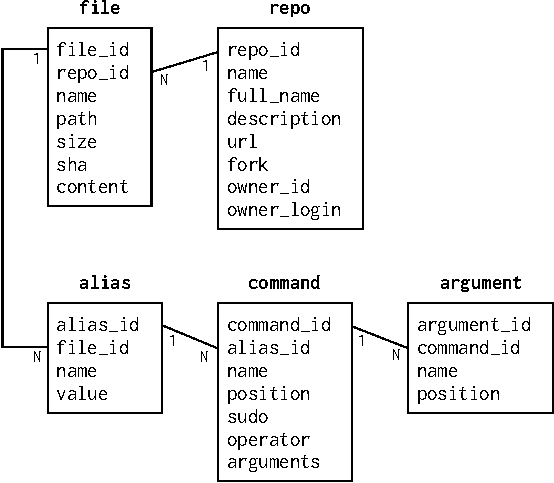
\includegraphics[width=0.9\columnwidth]{figures/schema.pdf}
    \caption{Relational database schema.}
    \label{fig:schema}
\end{figure}

The parser is a Haskell script that splits each alias definition into alias name and alias value, and tokenizes the value into commands and arguments.
Commands can be delimited by the shell operators for piping (\verb!|! and \verb!|&!), logical composition (\verb|&&| and \verb!||!), background execution (\verb|&|) and simple chaining (\verb|;|).
Arguments are separated by whitespace, but care is taken to handle quoted arguments correctly. 
For example, 
\begin{CVerbatim}
echo "hello world"
\end{CVerbatim}
is parsed as one command (\texttt{echo}) with one argument (\texttt{"hello world"}).
See \Cref{fig:parser} for a more elaborate example.

Beyond quoting, which is defined by the Shell Command Language and thus uniform across all commands, the parser can not make any further considerations as to how arguments are meant to be interpreted.
While there are some conventions around command line argument handling, programs are generally free to do as they wish and there is a wide variety of argument styles in the wild:
single-dash short arguments combined with double-dash long-form arguments (e.g., \texttt{ls -l -a --color=always});
combined short arguments without a dash (e.g., \texttt{tar xvzf archive.tar});
dictionary-style arguments (e.g., \texttt{dd if=/dev/zero of=/dev/sda});
subcommands (e.g., \texttt{git commit -m "wip"});
and many more.
Since the parser can not know the intentions of any command, it simply treats each token as a separate argument.
There is one exception: if the command is \cmd{sudo}, then its first argument is taken as the real command. 
For example,
\begin{CVerbatim}
sudo apt-get install
\end{CVerbatim} 
is parsed as the command \cmd{apt-get} with argument \texttt{install} and the sudo flag set.

After parsing, we ended up with \num{2204199} alias definitions, broken down into \num{2534167} commands and \num{3630423} arguments.
Files that did not contain any aliases were removed from the database, as was repository metadata that only referenced files without aliases.
\num{194218} files from \num{138112} repositories, or \per{52.09} of the original sample without duplicates, contained aliases.
%The majority of aliases in our dataset (\per{86.2}) originate from common startup scripts, like \texttt{.bashrc} or \texttt{.profile} (see \Cref{tab:file-names}).
% TODO: explain the renaming 14%

%\begin{table}
	\caption{Distribution of common file names}
    \label{tab:file-names}
    \begin{tabular}{rrlll}
        \toprule
                  \% &         Files &           Name Pattern &        Aliases &           \% \\
        \midrule
         \num{14.55} &  \num{28255}  &         \verb|*alias*| &  \num{626071}  &   \num{28.4} \\
         \num{27.73} &  \num{53855}  &        \verb|*bashrc*| &  \num{591482}  &  \num{26.83} \\
         \num{22.15} &  \num{43011}  &         \verb|*zshrc*| &  \num{487002}  &  \num{22.09} \\
          \num{9.42} &  \num{18305}  &       \verb|*profile*| &  \num{199168}  &   \num{9.04} \\
        \bottomrule
        \end{tabular}
\end{table}

\subsection{Reproducibility}
\label{sec:reproducibility}

To enable reproducibility and follow-up studies, we have made all data and our entire tool-chain publicly available.
Our dataset (1.45 GB of parsed alias definitions, plus 4.3 GB unparsed file contents and metadata) is available on Zenodo.\footnote{\url{https://doi.org/10.5281/zenodo.4007049}}
The parsing script and the executable Jupyter notebooks, containing all SQL queries and additional Python code used during our analysis, are available on GitHub.\footnote{Omitted for double blind review.}
%\footnote{\url{https://github.com/ipa-lab/shell-alias-analysis}}
